\subsection*{Punto de equilibrio}
\addcontentsline{toc}{subsection}{Punto de equilibrio}

Es importante calcular el punto de equilibrio, ya que permite a la empresa conocer cuántas unidades debe vender para cubrir los costos fijos en los que incurre durante sus operaciones. Asimismo, resulta fundamental determinar en qué momento las ventas comienzan a generar ganancias para la empresa. En la tabla \ref{CostosFijos} se proyectan los costos fijos y variables correspondientes a las ventas del primer año de operación.

\begin{table}[H]
	\centering
	\caption[{Costos fijos y variables}]{\centering Costos fijos y variables. \textit{Fuente:} Autores.}
	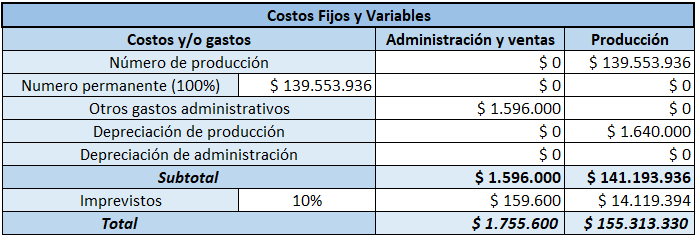
\includegraphics[width=13cm]{Imagenes/CostosFijos.png}
	\label{CostosFijos}
\end{table}

Se estima el costo fijo para producir cada unidad, en donde consideramos a cada unidad como un usuario de paga o gratuito que este en el servicio durante un mes, agregando el valor correspondiente a los costos administrativos y de ventas. A partir de esto, se proyecta un valor agregado del 19\% (\$503), con el fin de establecer un precio final de \$3.150. Con este valor, la plataforma debe tener un total de 3.490 suscripciones (314 de plan pago y las restantes del plan gratuito)  para recuperar la inversión realizada; a partir de ese punto, las ventas generarán utilidad.

\begin{table}[H]
	\centering
	\caption[{Estimaciones del punto de equilibrio}]{\centering Estimaciones del punto de equilibrio. \textit{Fuente:} Autores.}
	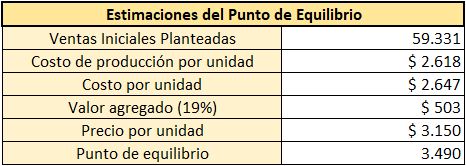
\includegraphics[width=11cm]{Imagenes/EstimacionesPunto.png}
	\label{EstimacionesPunto}
\end{table}

En la gráfica se observa el punto de equilibrio representado por las rectas de costos totales y de ventas. En el eje X se encuentra el número de unidades vendidas y en el eje Y la cantidad de dinero. De esta forma, se puede observar que con 3.490 suscripciones ambas rectas se intersectan, lo que corresponde al punto de equilibrio.

\begin{figure}[H]
	\centering
	\caption[{Gráfica del punto de equilibrio}]{\centering Gráfica del punto de equilibrio. \textit{Fuente:} Autores.}
	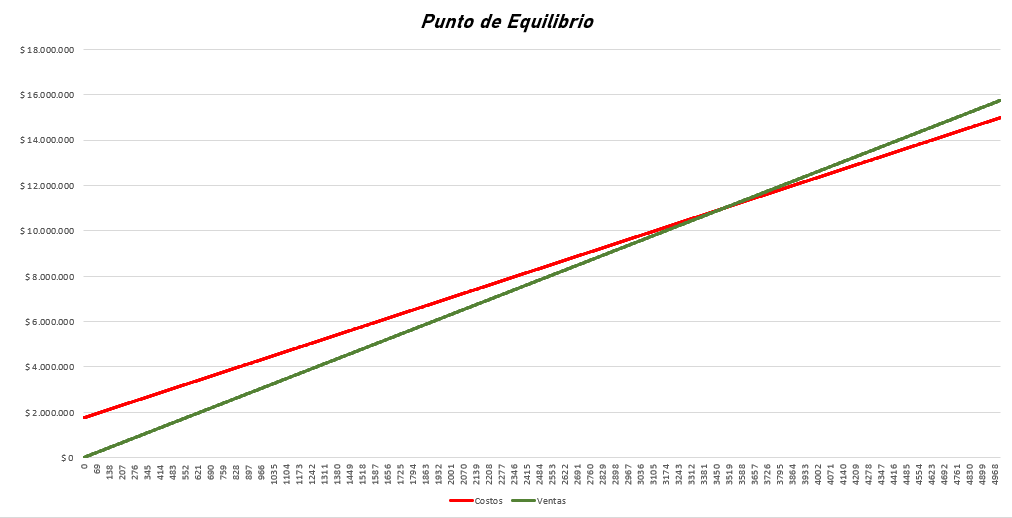
\includegraphics[width=15cm]{Imagenes/GraficaPunto.png}
	\label{fig:GraficaPunto}
\end{figure}

Finalmente, con base en los resultados anteriores, se presenta un resumen con la información necesaria para determinar el punto de equilibrio.

\begin{table}[H]
	\centering
	\caption[{Punto de equilibrio}]{\centering Punto de equilibrio. \textit{Fuente:} Autores.}
	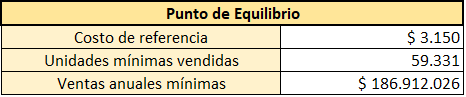
\includegraphics[width=10cm]{Imagenes/PuntoEquilibrio.png}
	\label{PuntoEquilibrio}
\end{table}